\begin{figure}%
\centering
\subfloat[Bone~Pin~Holder]{%
\label{subfig:pinHolder}%

\includegraphics[viewport=0 0 185pt 310pt]{figures/Blank}%
}%
\hspace{42pt}%
\captionsetup[subfigure]{justification=RaggedRight,singlelinecheck=false}%
\subfloat[Instrumented Holder]{%
\label{subfig:instrumentedHolder}%
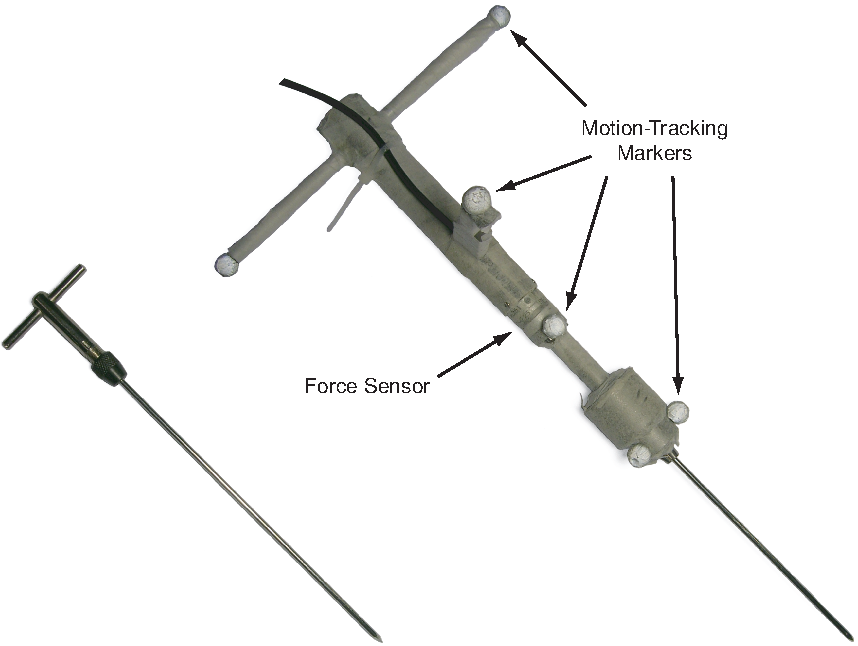
\includegraphics[viewport=227pt 0 412pt 310pt]{figures/PinHolders}%
}%
\caption[Pin insertion tools]{%
  Pin insertion tools (at \ensuremath{\sim}0.3\ensuremath{\times} scale). \subref{subfig:pinHolder} The bone pin is held in a T-handled pin vise. \subref{subfig:instrumentedHolder} To measure the force characteristics of the task, a pin holder was built that incorporated a force sensor and motion-tracking markers.%
}%
\label{fig:pinHolders}%
\end{figure}

If all the figures you ever want to include are rectangular, read no further.
Sometimes though, you have two figures that you want to present side-by-side, where allocating each one its own rectangle of space would be wasteful.
If that is the case, an easy hack is to use some program (like Illustrator) to combine the two figures in a nicely overlapping way.
But then how do you assign them subfigure labels?
You cheat!
\autoref{fig:pinHolders} is an example of this.
It may look like two different figures side-by-side\dots and it is!
But the figure on the left is actually a blank image.
We just messed around with the \texttt{viewport} argument to $\backslash$\texttt{includegraphics} so that the subfigure captions are nicely positioned. 